\subsubsection{Unsupervised Learning: Introduction}
\begin{itemize}[--]
	\item In supervised learning we're given a training set $\{(x^{(m)}, y^{(m)})\}$, we try and find the decision boundary
	\item In \textbf{unsupervised learning} we're given a training set $\{x^{(m)}\}$, give it to an algorithm and try and find structure
	\item An example is a clustering algorithm, which finds data that close together
	\item Applications of clusterin: market segmentation, social network analysis, organize computing clusters, astronomical data analysis
\end{itemize}

\subsubsection{K-Means Algorithm}
\begin{itemize}[--]
	\item Randomly initialize two points, called the \textbf{cluster centroids}
	\begin{center}
		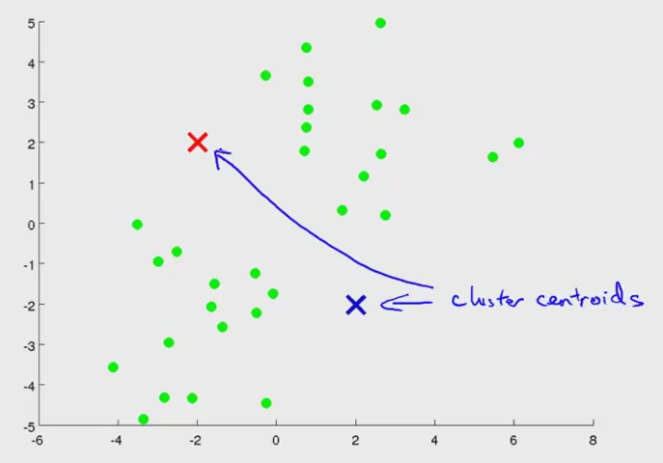
\includegraphics[scale=0.5]{sections/cs229/w10/kmeans1.png}
	\end{center}

	\item You should have a cluster centroid for each group you want 
	\item There's two steps: cluster assignment, and move centroid
	\item \textbf{Cluster assignment}: go through each example, and depending on which cluster it is closer to it will assign it to one of the centroids
	\begin{center}
		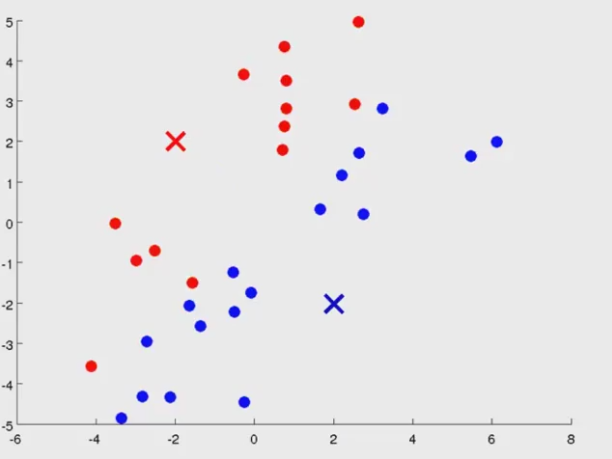
\includegraphics[scale=0.5]{sections/cs229/w10/kmeans2.png}
	\end{center}
	\item \textbf{Move centroid}: move the centroids to the mean of all the same groupped points
	\begin{center}
		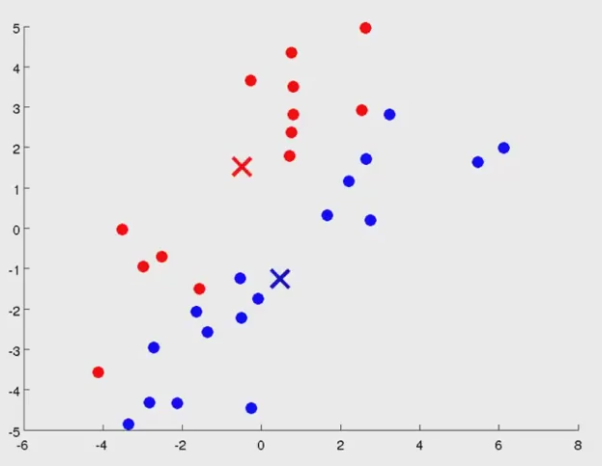
\includegraphics[scale=0.5]{sections/cs229/w10/kmeans3.png}
	\end{center}

	\item Then you repeat this process until the movement of the centroids
	\begin{center}
		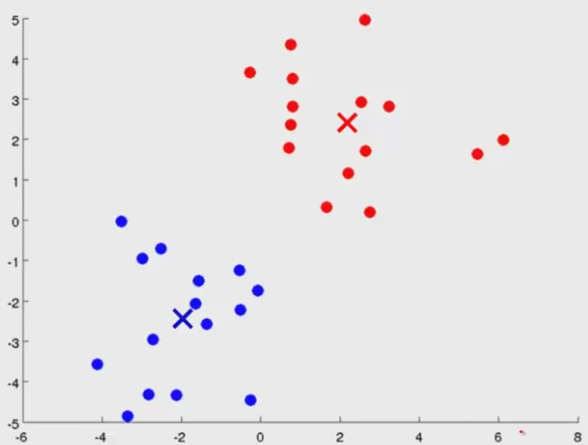
\includegraphics[scale=0.5]{sections/cs229/w10/kmeans4.png}
	\end{center}

	\item \textbf{$K$-means Algorithm}
	\begin{itemize}[--]
		\item Input:
		\begin{itemize}[--]
			\item $K$ (number of clusters)
			\item Training set $\{ x^{(1)}, \ldots, x^{(m)}\}$
		\end{itemize}
		\item $x^{(i)}\in\mathbb{R}^n $ (drop $x_0=1$ convention)
		\item Randomly initialize $K$ cluster centroids $\mu_1,\ldots, \mu_k \in\mathbb{R}^n$
		\item Repeat: TODO: pseudo-code markup
		\begin{itemize}[--]
			\item for $i=1$ to $m$
			\begin{itemize}[--]
				\item $c^{(i)} :=$ index (from 1 to $K$) of cluster centroid closest to $x^{(i)}$ ($\min_k ||x^{(i)} -\mu_k||^2$)
			\end{itemize}
			\item for $k=1$ to $K$
			\begin{itemize}[--]
				\item $\mu_k :=$ average (mean) of points assigned to cluster $k$
			\end{itemize}
		\end{itemize}
	\end{itemize}
\end{itemize}

\subsubsection{Optimization Objective}
\begin{itemize}[--]
	\item $\mu_c (i):=$ cluster centroid of cluster to which example $x^{(i)}$ has been asigned ($x^{(i)}\to 5$, $c^{(i)}=5$, $\mu_{c^{(i)}} =\mu_5$)
	\item Optimzation Objective:
		$$J(c^{(1)},\ldots, c^{(m)}, \mu_1,\ldots, \mu_K )=\frac{1}{m}\sum_{i=1}^{m}||x^{(i)}-\mu_{c^{(i)}}||^2$$
		$$\min_{c^{(1)},\ldots, c^{(m)}, \mu_1, \ldots, \mu_K} J(\ldots )$$
	\item The cluster assignment step, can be shown to be this minimization process of the cost function to the group assignment holding the centroids constant
	\item The moving centroids minimize with respect to the centroids
\end{itemize}

\subsubsection{Random Initialization}
\begin{itemize}[--]
	\item Instead of random centroids, randomly pick $K$ training examples, and set $\mu_1,\ldots, \mu_k$ be these $K$ examples
	\item There exists local optimum, to prevent this we may run the entire $K$-means algorithm, and choose the lowest cost solution
	\item If $K=2-10$, doing local random initializations to find optimal, works well; however, if $K$ is larger then this tends to fall apart
\end{itemize}

\subsubsection{Choosing the Number of Clusters}
\begin{itemize}[--]
	\item The most common way is to manually choose it based on observations.
	\item There exists situations, where it's ambiguous the true number of clusters:
	\begin{center}
		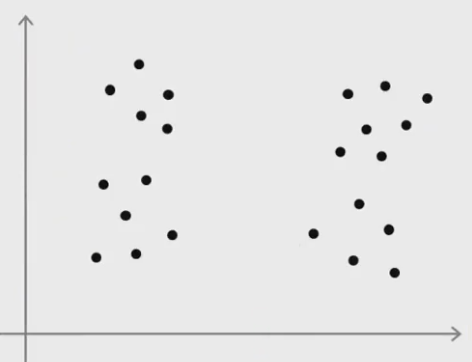
\includegraphics[scale=0.5]{sections/cs229/w10/amb.png}
	\end{center}

	\item The \textbf{elbow method} is to run $K$-means many times and vary the number of clusters.
	\begin{center}
		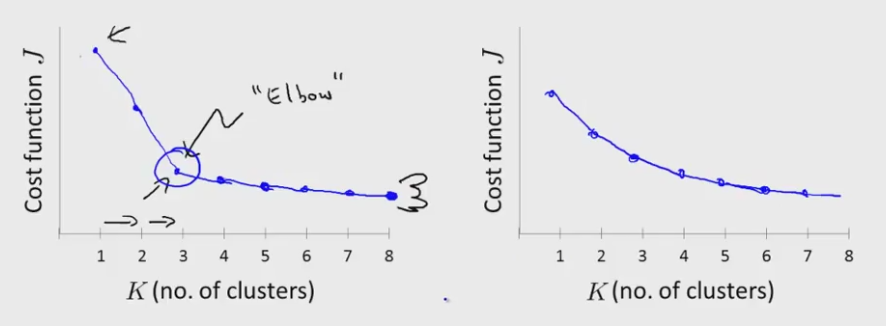
\includegraphics[scale=0.5]{sections/cs229/w10/elbow.png}
	\end{center}

	\item The method looks at the plot, and takes the ``elbow'' as the correct value
	\item The elbow method isn't typically used, because the curve can be just as ambiguous
	\item ``It's worth a shot, but don't have high expectations''
	\item Sometimes, you're running K-means to get clusters to ue for some later/downstream purpose. Evaluate K-means based on a metric for how well it performs for that later purpose
	\item 

\end{itemize}